% Section 2: Normed Vector Spaces  (original handwritten pages 11--18)
\section{Normed Vector Spaces}\label{sec:normed}
\syllabusweek{Week 3 --- normed spaces, sequences and convergence, matrix norms}

\subsection{Norms}\label{ss:norms}

\begin{definition}
Let $(\V,\F)$ be a vector space, a \term{norm} of $\V$ is a function shown as
\[ \norm{\cdot}: \V\to\R_{\ge0} \]
satisfying the following properties:
\begin{enumerate}[label=(N\arabic*),leftmargin=3.2em]
\item $\norm{v}\ge0 \quad \forall v\in\V$, \quad $\norm{v}=0 \iff v=0_{\V}$ \hfill (positive definiteness)
\item $\norm{\alpha v} = \abs{\alpha}\norm{v} \quad \forall v\in\V\ \&\ \forall\alpha\in\F$ \hfill (absolute homogeneity)
\item $\norm{v_1+v_2}\le\norm{v_1}+\norm{v_2} \quad \forall v_1,v_2\in\V$ \hfill (triangle inequality)
\end{enumerate}
The triplet $(\V,\F,\norm{\cdot})$ is called a \term{normed space}.
\end{definition}
\begin{align*}
&\norm{v} = \norm{v-0_{\V}}: && \text{size of } v\\
&\norm{v_1-v_2}: && \text{distance between } v_1 \ \&\ v_2
\end{align*}
We can define a sphere in $\V$:
\[
S = \{ v\in\V \mid \norm{v-v_0}\le r\} \qquad \text{sphere radius } r,\quad v_0: \text{center vector}
\]
\explain{Strictly, with ``$\le$'' this is the (closed) \term{ball}; the sphere is its boundary $\norm{v-v_0}=r$. The ``unit spheres'' drawn below are the sets $\norm{x}=1$.}

\begin{example}
$\V=\R^n$, $\F=\R$
\[
x = \bmat{x_1\\\vdots\\x_n}, \qquad \norm{x}_1 \overset{?}{=} \sum_{i=1}^{n}\abs{x_i}
\]
\paragraph{(N1).} $\abs{x_i}\ge0\ \forall i \Rightarrow \norm{x}_1\ge0$ \ $\checkmark$. \quad $0_{\V} = (0,\dots,0)\T$; if $\norm{x}_1=0$:
\[
\norm{x}_1 = \sum_{i=1}^{n}\abs{x_i} = 0
\ \Rightarrow\ \abs{x_i}=0 \ \forall i
\ \Rightarrow\ x=0_{\V}
\]
\paragraph{(N2).} $\alpha x = (\alpha x_1,\, \alpha x_2,\, \dots,\, \alpha x_n)\T$:
\begin{align*}
\norm{\alpha x}_1 &= \sum_{i=1}^{n}\abs{\alpha x_i} = \sum_{i=1}^{n}\abs{\alpha}\cdot\abs{x_i}
= \abs{\alpha}\cdot\underbrace{\sum_{i=1}^{n}\abs{x_i}}_{\norm{x}_1} = \abs{\alpha}\norm{x}_1
\end{align*}

% ===== Page 11 =====
\needspace{8\baselineskip}
\paragraph{(N3).} $x+y = (x_1+y_1,\, x_2+y_2,\, \dots,\, x_n+y_n)\T$:\origpage{11}
\begin{align*}
\norm{x+y}_1 = \sum_{i=1}^{n}\abs{x_i+y_i} &\le \sum_{i=1}^{n}\left(\abs{x_i}+\abs{y_i}\right)
= \underbrace{\sum_{i=1}^{n}\abs{x_i}}_{\norm{x}_1}+\underbrace{\sum_{i=1}^{n}\abs{y_i}}_{\norm{y}_1}
\end{align*}
% corrected: notes had \norm{x_i} in (1) and the sum without parentheses in (3)
\explain{The inequality uses the scalar triangle inequality $\abs{x_i+y_i}\le\abs{x_i}+\abs{y_i}$ term by term. Hence $\norm{x+y}_1\le\norm{x}_1+\norm{y}_1$ and all three properties hold: $\norm{\cdot}_1$ is a norm.}
\end{example}

\subsection{The $\ell_p$ Norms and Unit Spheres}\label{ss:lp}
\point $\norm{\cdot}_1$ is called \term{$\ell_1$ norm}.

\begin{example}[$\ell_2$ norm]
\[
\norm{x}_2 = \sqrt{\sum_{i=1}^{n}\abs{x_i}^2} = \left(\sum_{i=1}^{n}\abs{x_i}^2\right)^{1/2}
\]
Unit spheres for $x = (x_1,x_2)\T$: \ $\norm{x}_2=1$ and $\norm{x}_1 = 1$.

For $\ell_1$ norm: $\abs{x_1}+\abs{x_2}=1$
\begin{itemize}[nosep]
\item 1st quadrant ($x_1,x_2\ge0$): $x_1+x_2=1$
\item 2nd quadrant ($x_1\le0\le x_2$): $-x_1+x_2=1$
\item 3rd quadrant ($x_1,x_2\le0$): $-x_1-x_2=1$
\item 4th quadrant ($x_2\le0\le x_1$): $x_1-x_2=1$
\end{itemize}
% corrected: notes had "1st quadrant: x_1 - x_2 = 1"; in the 1st quadrant |x_1|+|x_2| = x_1+x_2. 3rd/4th quadrants added.
\explain{Four line segments joining $(\pm1,0)$ and $(0,\pm1)$: the $\ell_1$ unit sphere is a diamond (a square rotated by $45^\circ$), while the $\ell_2$ unit sphere $x_1^2+x_2^2=1$ is the circle.}
\begin{center}
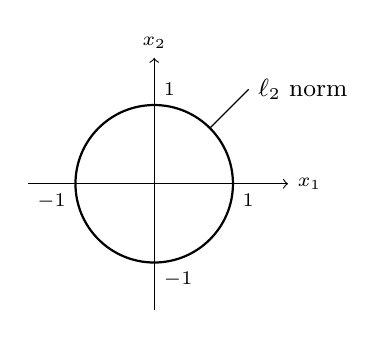
\begin{tikzpicture}[scale=1.0]
\draw[->] (-1.6,0) -- (1.7,0) node[right] {\scriptsize$x_1$};
\draw[->] (0,-1.6) -- (0,1.6) node[above] {\scriptsize$x_2$};
\draw[thick] (0,0) circle (1);
\node[below left] at (-1,0) {\scriptsize$-1$};
\node[below right] at (1,0) {\scriptsize$1$};
\node[above right] at (0,1) {\scriptsize$1$};
\node[below right] at (0,-1) {\scriptsize$-1$};
\draw (0.707,0.707) -- (1.2,1.2) node[right] {\small$\ell_2$ norm};
\end{tikzpicture}
\qquad\qquad
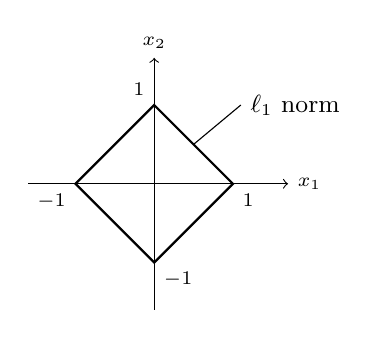
\begin{tikzpicture}[scale=1.0]
\draw[->] (-1.6,0) -- (1.7,0) node[right] {\scriptsize$x_1$};
\draw[->] (0,-1.6) -- (0,1.6) node[above] {\scriptsize$x_2$};
\draw[thick] (1,0) -- (0,1) -- (-1,0) -- (0,-1) -- cycle;
\node[below left] at (-1,0) {\scriptsize$-1$};
\node[below right] at (1,0) {\scriptsize$1$};
\node[above left] at (0,1) {\scriptsize$1$};
\node[below right] at (0,-1) {\scriptsize$-1$};
\draw (0.5,0.5) -- (1.1,1.0) node[right] {\small$\ell_1$ norm};
\end{tikzpicture}
\end{center}
\end{example}

\paragraph{$\ell_p$ norm.} The \term{$\ell_p$ norm} is
\[
\norm{x}_p = \left(\sum_{i=1}^{n}\abs{x_i}^p\right)^{1/p} \quad\text{where } p\ge1
\]
\paragraph{$\ell_\infty$ norm.} The \term{$\ell_\infty$ norm} is
\[
\norm{x}_\infty = \max_i\abs{x_i} = \lim_{p\to\infty}\norm{x}_p
\]
\needspace{9\baselineskip}
For $\V=\R^2$: $x=(x_1,x_2)\T$, \ $\norm{x}_p = \left(\abs{x_1}^p+\abs{x_2}^p\right)^{1/p}$. For $x_1=2$ \& $x_2=3$:
\begin{align*}
\norm{\bmat{2\\3}}_p &= (2^p+3^p)^{1/p}\\
&= (3^p)^{1/p}\cdot\left(1+\left(\tfrac23\right)^p\right)^{1/p}\\
&= 3\left(1+\left(\tfrac23\right)^p\right)^{1/p}\\
\lim_{p\to\infty}\norm{\bmat{2\\3}}_p &= 3 = \max\left(\abs{x_1},\abs{x_2}\right) = \norm{\bmat{2\\3}}_\infty
\end{align*}
\explain{$\left(\tfrac23\right)^p\to0$, so the factor $\left(1+(\tfrac23)^p\right)^{1/p}\to1$. In general the largest $\abs{x_i}$ dominates the sum: $\max_i\abs{x_i}\le\norm{x}_p\le n^{1/p}\max_i\abs{x_i}$ and $n^{1/p}\to1$.}

\sep
\point Unit spheres $\norm{x}_p=1$, i.e.\ $\norm{x-0_{\V}}_p=1$. The $\ell_\infty$ unit sphere is $\max(\abs{x_1},\abs{x_2}) = 1$.
\begin{center}
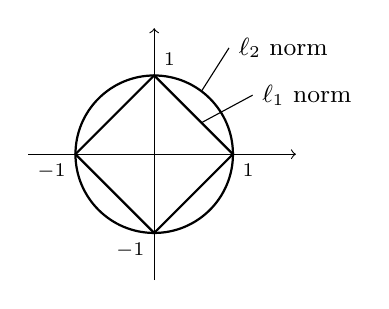
\begin{tikzpicture}[scale=1.0]
\draw[->] (-1.6,0) -- (1.8,0);
\draw[->] (0,-1.6) -- (0,1.6);
\draw[thick] (0,0) circle (1);
\draw[thick] (1,0) -- (0,1) -- (-1,0) -- (0,-1) -- cycle;
\node[below left] at (-1,0) {\scriptsize$-1$};
\node[below right] at (1,0) {\scriptsize$1$};
\node[above right] at (0,1) {\scriptsize$1$};
\node[below left] at (0,-1) {\scriptsize$-1$};
\draw (0.6,0.8) -- (0.95,1.35) node[right] {\small$\ell_2$ norm};
\draw (0.6,0.4) -- (1.25,0.75) node[right] {\small$\ell_1$ norm};
\end{tikzpicture}
\qquad\qquad
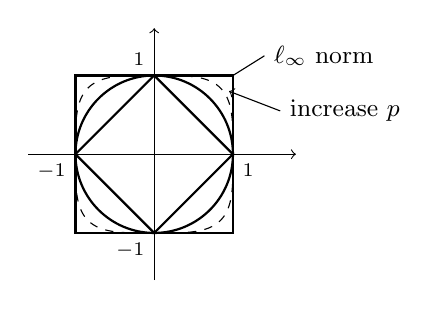
\begin{tikzpicture}[scale=1.0]
\draw[->] (-1.6,0) -- (1.8,0);
\draw[->] (0,-1.6) -- (0,1.6);
\draw[thick] (-1,-1) rectangle (1,1);
\draw[thick] (0,0) circle (1);
\draw[thick] (1,0) -- (0,1) -- (-1,0) -- (0,-1) -- cycle;
% intermediate p (p = 4): |x1|^4 + |x2|^4 = 1
\draw[dashed,domain=0:360,samples=145,smooth,variable=\t]
  plot ({sign(cos(\t))*abs(cos(\t))^(0.5)},{sign(sin(\t))*abs(sin(\t))^(0.5)});
\node[below left] at (-1,0) {\scriptsize$-1$};
\node[below right] at (1,0) {\scriptsize$1$};
\node[above left] at (0,1) {\scriptsize$1$};
\node[below left] at (0,-1) {\scriptsize$-1$};
\draw (1,1) -- (1.4,1.25) node[right] {\small$\ell_\infty$ norm};
\draw[->] (1.6,0.55) node[right] {\small increase $p$} -- (0.95,0.8);
\end{tikzpicture}
\end{center}
\explain{Dashed curve: $\abs{x_1}^p+\abs{x_2}^p=1$ for an intermediate $p$ (drawn for $p=4$); as $p$ increases the unit sphere moves from the $\ell_2$ circle towards the $\ell_\infty$ square.}

\sep
For $p=1/2$:
\[
\norm{x}_{1/2} = \left(\abs{x_1}^{1/2}+\abs{x_2}^{1/2}\right)^2
\]
\explain{It satisfies (N1) \& (N2) but need not satisfy the triangle inequality (N3).}
\paragraph{Counterexample.}
\[
x=\bmat{9\\0}, \quad y=\bmat{0\\4}, \quad x+y=\bmat{9\\4}
\]
\begin{align*}
\norm{x+y}_{1/2} &= \left(\sqrt9+\sqrt4\right)^2 = 25\\
\norm{x}_{1/2}&=9, \qquad \norm{y}_{1/2}=4\\
\norm{x+y}_{1/2} &\not\le \norm{x}_{1/2}+\norm{y}_{1/2}
\end{align*}
\[ \key{$p<1 \ \Rightarrow\ \text{no norms!}$} \]
\explain{Here $25>9+4=13$. Geometrically, for $p<1$ the ``unit sphere'' $\abs{x_1}^p+\abs{x_2}^p=1$ is star-shaped (curved inwards) and the unit ball is not convex; \key{a norm's unit ball is always convex}.}

% ===== Page 12 =====
\subsection{Norms on Function Spaces}\label{ss:function-norms}
\begin{center}\origpage{12}
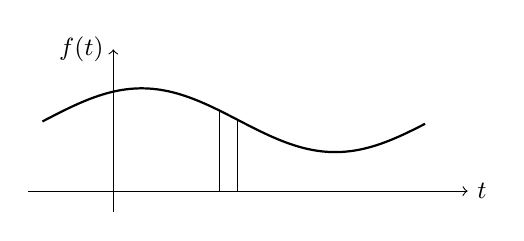
\begin{tikzpicture}[scale=0.9]
\draw[->] (-1.2,0) -- (5,0) node[right] {\small$t$};
\draw[->] (0,-0.3) -- (0,2) node[left] {\small$f(t)$};
\draw[thick,smooth,domain=-1:4.4,samples=60] plot (\x,{1.0+0.45*cos(deg(1.15*(\x-0.4)))});
% thin strip under the curve
\draw (1.5,0) -- (1.5,{1.0+0.45*cos(deg(1.15*1.1))});
\draw (1.75,0) -- (1.75,{1.0+0.45*cos(deg(1.15*1.35))});
\end{tikzpicture}
\end{center}
\[
\mathcal{L}_p = \left\{ f(\cdot) \;\middle|\; f:\R\to\R \text{ such that } \int_{-\infty}^{\infty}\abs{f(t)}^p\,dt<\infty \right\}, \qquad 1\le p<\infty
\]
\needspace{10\baselineskip}
\begin{align*}
\norm{f(t)}_p &= \left(\int_{-\infty}^{\infty}\abs{f(t)}^p\,dt\right)^{1/p} && \mathcal{L}_p \text{ norm}\\
\norm{f(t)}_1 &= \int_{-\infty}^{\infty}\abs{f(t)}\,dt && \mathcal{L}_1 \text{ norm}\\
\norm{f(t)}_2 &= \left(\int_{-\infty}^{\infty}\abs{f(t)}^2\,dt\right)^{1/2} && \mathcal{L}_2 \text{ norm}\\
\norm{f(t)}_\infty &= \sup_t\abs{f(t)} && \mathcal{L}_\infty \text{ norm}
\end{align*}
% corrected: notes had the L_p and L_2 integrals without dt, the L_1 norm without subscript, and max_t |f(t)| for L_infinity; the example below shows why sup is needed
\explain{These are the continuous analogues of the $\ell_p$ norms: the sum over $i$ becomes an integral over $t$.}

\sep
\needspace{12\baselineskip}
\begin{center}
$f(t) = 1-e^{-t},\quad t\ge0$
\qquad
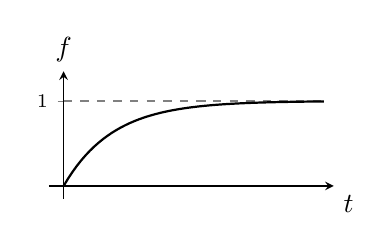
\begin{tikzpicture}[baseline=0.4cm]
\begin{axis}[width=5.2cm,height=3.2cm,axis lines=middle,xmin=-0.3,xmax=5.5,ymin=-0.15,ymax=1.35,
  xtick=\empty,ytick={1},xlabel={$t$},ylabel={$f$},
  xlabel style={anchor=north west},ylabel style={anchor=south},tick label style={font=\scriptsize}]
\addplot[dashed,gray,domain=0:5.3] {1};
\addplot[thick,domain=0:5.3,samples=60] {1-exp(-x)};
\end{axis}
\end{tikzpicture}
\end{center}
\explain{Value 1 is never reached. A maximum would have to be attained at a finite $t$, so $\max_t\abs{f(t)}$ does not exist here.}
The supremum, however, does exist:
\[ \sup_t\abs{f(t)} = 1 \quad (\text{least upper bound}) \]
\explain{Therefore \key{$\norm{f}_\infty$ is defined with $\sup$} (it always exists for bounded $f$), which equals $\max$ whenever the maximum is attained.}

\sep
\key{Integral norms do not satisfy $\norm{x}=0 \iff x=0_{\V}$!}
\begin{center}
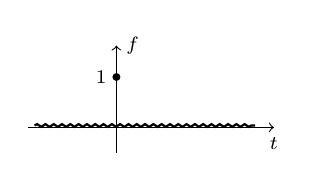
\begin{tikzpicture}[scale=0.8,baseline=0.2cm]
\draw[->] (-1.4,0) -- (2.5,0) node[below] {\scriptsize$t$};
\draw[->] (0,-0.4) -- (0,1.3) node[right] {\scriptsize$f$};
\fill (0,0.8) circle (1.8pt);
\node[left] at (0,0.8) {\scriptsize1};
\draw[thick,decorate,decoration={snake,amplitude=0.5pt,segment length=3pt}] (-1.3,0.03) -- (2.2,0.03);
\end{tikzpicture}
\qquad
$f(t) = \begin{cases} 1, & t=0\\ 0, & \text{otherwise}\end{cases}
\qquad\Rightarrow\qquad
\displaystyle\int_{-\infty}^{\infty}\abs{f(t)}\,dt = 0$
\end{center}
\explain{Such functions are equivalent to the zero function, as they take nonzero values only at finitely many points.}
\begin{insight}[How this is fixed]
$f\neq0$ but $\norm{f}_1=0$, so property (N1) fails on the set of all functions. The standard remedy: regard two functions as \emph{equal} in $\mathcal{L}_p$ if they differ only on a set of zero length (e.g.\ finitely many points), i.e.\ if $\norm{f-g}_p=0$. With this identification $\norm{\cdot}_p$ is a genuine norm on $\mathcal{L}_p$ for $p\ge1$ (the triangle inequality is Minkowski's inequality).
\end{insight}

\subsection{Matrix Norms}\label{ss:matrix-norms}
\[ A = \bmat{1&-2\\3&4}, \qquad \norm{A}=\,? \]

\subsubsection{Entrywise Norms (Frobenius)}
\needspace{14\baselineskip}
\paragraph{1st method.}
\[
\operatorname{Vec}(A) \triangleq \bmat{1\\3\\-2\\4}, \qquad A = \bmat{a_{11}&a_{12}\\a_{21}&a_{22}}
\]
\begin{align*}
\norm{A}_p = \norm{\operatorname{Vec}(A)}_p = \norm{\bmat{1\\3\\-2\\4}}_p &= \left(\abs{1}^p+\abs{3}^p+\abs{-2}^p+\abs{4}^p\right)^{1/p}\\
&= \left(\sum_{i,j}\abs{a_{ij}}^p\right)^{1/p}, \qquad p\ge1
\end{align*}
\begin{insight}[Numbers for this $A$]
\[
\norm{A}_1 = 1+2+3+4 = 10, \quad
\norm{A}_2 = \sqrt{1+4+9+16}=\sqrt{30}\approx5.48, \quad
\norm{A}_\infty = \max_{i,j}\abs{a_{ij}} = 4
\]
The case $p=2$ is the \term{Frobenius norm} $\norm{A}_F$. Since $\R^{m\times n}$ is a vector space that is identified with $\R^{mn}$ through $\operatorname{Vec}$, every vector norm gives a matrix norm in this way.
\end{insight}

% ===== Page 13 =====
\origpage{13}
\paragraph{1st method (Frobenius norm).}
% consistency: notes wrote ||A||_2 here; renamed ||A||_F as in the insight below (||A||_2 is reserved for the induced 2-norm)
\begin{align*}
\norm{A}_F &= \Big(\sum_{i,j} |a_{ij}|^2\Big)^{1/2} && \text{(\term{Frobenius norm})}\\
&= \sqrt{\tr(A\T A)} && \text{(real)}\\
&= \sqrt{\tr(A\Hm A)} && \text{(complex)}
\end{align*}
For example, with
\[
A = \bmat{a_{11} & a_{12}\\ a_{21} & a_{22}},
\qquad
A\T A = \underbrace{\bmat{a_{11} & a_{21}\\ a_{12} & a_{22}}}_{A\T}
\underbrace{\bmat{a_{11} & a_{12}\\ a_{21} & a_{22}}}_{A}
= \bmat{a_{11}^2 + a_{21}^2 & \\ & a_{12}^2 + a_{22}^2}
\]
% corrected: notes had tr(A) on the left-hand side (the trace taken is that of A^T A)
\needspace{5\baselineskip}
\begin{align*}
\tr(A\T A) &= a_{11}^2 + a_{21}^2 + a_{12}^2 + a_{22}^2\\*
&= \sum_{i,j} a_{ij}^2
\end{align*}
\explain{Only the diagonal of $A\T A$ matters for the trace, so its off-diagonal entries ($a_{11}a_{12}+a_{21}a_{22}$) are left blank.}
\begin{insight}
In general $(A\Hm A)_{jj} = \sum_i \overline{a_{ij}}\,a_{ij} = \sum_i |a_{ij}|^2$ is the squared length of the $j$-th column of $A$, so
$\tr(A\Hm A) = \sum_j\sum_i |a_{ij}|^2$. The Frobenius norm is simply the Euclidean norm of $A$ viewed as a long vector in $\F^{mn}$; we write it $\norm{A}_F$ to distinguish it from the \emph{induced} $2$-norm of the 2nd method below (which is in general different, e.g.\ $\norm{I_n}_F = \sqrt n$ but the induced norm of $I_n$ is $1$).
\end{insight}

\subsubsection{Induced Matrix Norms}
\paragraph{2nd method (induced norm).} Measure $A$ through its action on vectors.
\begin{definition}
Let $A:\R^n \to \R^m$ be an $m\times n$ matrix. Let $\norm{\cdot}_{\R^n}$ and $\norm{\cdot}_{\R^m}$ denote the norms in $\R^n$ \& $\R^m$ respectively. The \term{induced matrix norm} is defined as
\[
\norm{A} \triangleq \max_{\substack{x\in\R^n\\ x\neq 0_{\V}}} \frac{\norm{Ax}_{\R^m}}{\norm{x}_{\R^n}}
\]
\end{definition}
\[
\underbrace{\bmat{a_{11} & \cdots & a_{1n}\\ \vdots & \ddots & \vdots\\ a_{m1} & \cdots & a_{mn}}}_{A}
\underbrace{\bmat{x_1\\ \vdots\\ x_n}}_{x}
=
\underbrace{\bmat{y_1\\ \vdots\\ y_m}}_{y}
\]

\paragraph{Why second method?}
\begin{align*}
|\inner{x}{y}| &\le \norm{x}\norm{y}\\
\norm{Ax} &\le \norm{A}\norm{x}\\
\norm{Ax} &= \frac{\norm{Ax}}{\norm{x}}\cdot\norm{x} \le \left(\max\frac{\norm{Ax}}{\norm{x}}\right)\cdot\norm{x} = \norm{A}\norm{x}
\end{align*}
\explain{``Cauchy--Schwarz''-like inequality for matrices: \key{$\norm{Ax}\le\norm{A}\norm{x}$ for every $x$}.}
\begin{insight}[Why the induced norm is useful]
The induced norm is the largest ``gain'' $\norm{Ax}/\norm{x}$ of $A$, so $\norm{Ax}\le\norm{A}\norm{x}$ holds for every $x$ with the smallest possible constant. It is also submultiplicative: $\norm{ABx}\le\norm{A}\norm{Bx}\le\norm{A}\norm{B}\norm{x}$, hence $\norm{AB}\le\norm{A}\norm{B}$, which is what makes it convenient for bounding $\lVert A^k\rVert$ in system analysis.
\end{insight}

\begin{align*}
\norm{A} &= \max_{\substack{x\in\R^n\\ x\neq 0_{\V}}} \norm{A\frac{x}{\norm{x}_{\R^n}}}_{\R^m}\\
&= \max_{\norm{x}_{\R^n}=1} \norm{Ax}_{\R^m}
\end{align*}
\explain{First step: absolute homogeneity of the norm, $\frac{\norm{Ax}}{\norm{x}} = \norm{A\frac{x}{\norm{x}}}$, and $\frac{x}{\norm{x}}$ ranges over all unit vectors.}
\needspace{10\baselineskip}
\begin{keybox}
\[
\therefore\ \norm{A} = \max_{\norm{x}_{\R^n}=1} \norm{Ax}_{\R^m}
\]
\end{keybox}
\begin{center}
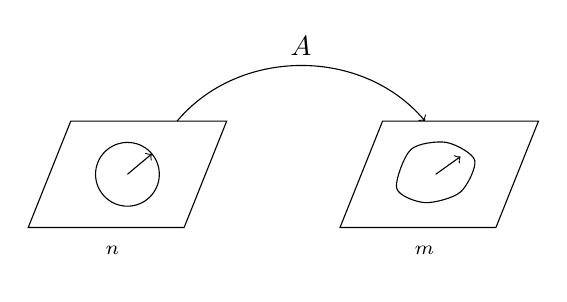
\begin{tikzpicture}[scale=0.9]
  % R^n parallelogram with unit ball
  \draw (0,0) -- (2.2,0) -- (2.8,1.5) -- (0.6,1.5) -- cycle;
  \draw (1.4,0.75) circle (0.45);
  \draw[->] (1.4,0.75) -- ++(40:0.45);
  \node at (1.2,-0.4) {$\R^n$};
  % R^m parallelogram with image of the unit ball
  \draw (4.4,0) -- (6.6,0) -- (7.2,1.5) -- (5.0,1.5) -- cycle;
  \draw plot[smooth cycle] coordinates {(5.2,0.55) (5.6,0.35) (6.1,0.5) (6.3,0.95) (5.9,1.2) (5.4,1.1)};
  \draw[->] (5.75,0.75) -- (6.1,1.0);
  \node at (5.6,-0.4) {$\R^m$};
  % mapping arrow
  \draw[->] (2.1,1.5) to[out=50,in=130] node[above] {$A$} (5.6,1.5);
\end{tikzpicture}
\end{center}

% ===== Page 14 =====
\origpage{14}
\begin{example}
Consider an $m\times n$ matrix with real elements. Choose $\ell_\infty$-norm $\norm{\cdot}_\infty$ for both $\R^n$ \& $\R^m$.
\[
\norm{A}_\infty = \max_{\norm{x}_\infty=1} \norm{Ax}_\infty,
\qquad
A = \bmat{1 & -2\\ -3 & 4\\ -2 & 2},
\qquad x\in\R^2,\quad y = Ax \in \R^3
\]
\[
\norm{x}_\infty = \max(|x_1|,|x_2|) = 1
\]
\begin{center}
\begin{minipage}{0.4\textwidth}
\centering
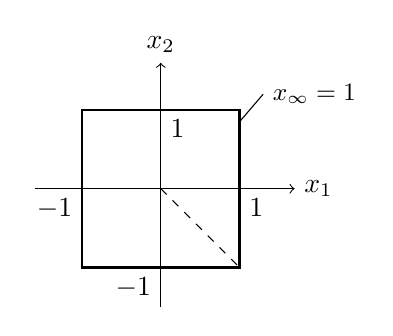
\begin{tikzpicture}[scale=1.0]
  \draw[->] (-1.6,0) -- (1.7,0) node[right] {$x_1$};
  \draw[->] (0,-1.5) -- (0,1.6) node[above] {$x_2$};
  \draw[thick] (-1,-1) rectangle (1,1);
  \node[below left] at (-1,0) {$-1$};
  \node[below right] at (1,0) {$1$};
  \node[below right] at (0,1) {$1$};
  \node[below left] at (0,-1) {$-1$};
  \draw[dashed] (0,0) -- (1,-1);
  \draw (1,0.85) -- (1.3,1.2) node[right,font=\small] {$\norm{x}_\infty=1$};
\end{tikzpicture}
\end{minipage}%
\begin{minipage}{0.55\textwidth}
First row only:
\[
A_1 = \bmat{1 & -2}\bmat{x_1\\ x_2}
\]
\[
\max_{\norm{x}_\infty=1} |A_1 x| = \max_{\norm{x}_\infty=1} |x_1 - 2x_2| = 3
\]
\explain{Attained at $x_1 = 1$, $x_2 = -1$ (dashed corner).}
\end{minipage}
\end{center}
For the whole matrix:
\begin{align*}
Ax &= \bmat{x_1 - 2x_2\\ -3x_1 + 4x_2\\ -2x_1 + 2x_2}\\
\norm{Ax}_\infty &= \max\big(|x_1 - 2x_2|,\ |-3x_1+4x_2|,\ |-2x_1+2x_2|\big)\\
x^* &= \bmat{1\\ -1} \quad\text{or}\quad x^* = \bmat{-1\\ 1}\\
Ax^* &= \bmat{3\\ -7\\ -4} \;\Rightarrow\; \norm{Ax^*}_\infty = 7
\end{align*}
\[
\boxed{\norm{A}_\infty = 7}
\]
\end{example}
\needspace{11\baselineskip}
\begin{keybox}
\[
\norm{A}_\infty = \max_i \sum_{j=1}^n |a_{ij}| \qquad \text{(max row sum)}
\]
\end{keybox}
\begin{insight}[Why the max row sum]
If $\norm{x}_\infty = 1$ then $|x_j|\le 1$ for all $j$, so for each row
$|(Ax)_i| = \big|\sum_j a_{ij}x_j\big| \le \sum_j |a_{ij}||x_j| \le \sum_j |a_{ij}|$.
Hence $\norm{Ax}_\infty\le\max_i\sum_j|a_{ij}|$. Equality is reached by taking the row $i^*$ with the largest sum and $x_j = \operatorname{sign}(a_{i^*j})$ (a corner of the square). In the example the row sums are $3,7,4$ and row 2 $= [-3\ \ 4]$ gives $x^* = [-1\ \ 1]\T$ (or its negative).
\end{insight}

\sep
\paragraph{$\ell_1$-norm.}
\[
\norm{A}_1 = \max_{\norm{x}_1=1}\norm{Ax}_1, \qquad \norm{x}_1 = |x_1| + |x_2| = 1
\]
\begin{center}
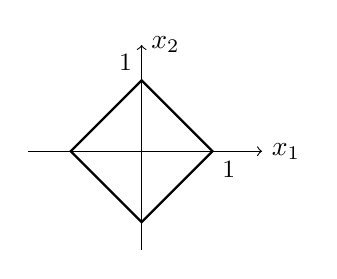
\begin{tikzpicture}[scale=0.9]
  \draw[->] (-1.6,0) -- (1.7,0) node[right] {$x_1$};
  \draw[->] (0,-1.4) -- (0,1.5) node[right] {$x_2$};
  \draw[thick] (1,0) -- (0,1) -- (-1,0) -- (0,-1) -- cycle;
  \node[below right,font=\small] at (1,0) {$1$};
  \node[above left,font=\small] at (0,1) {$1$};
\end{tikzpicture}
\end{center}
\begin{align*}
A_1 &= \bmat{1 & -2}\\
A_1 x &= x_1 - 2x_2\\
\norm{A_1 x} &= |x_1 - 2x_2|\\
\max_{\norm{x}_1 = 1}\norm{A_1 x} &= \max_{\norm{x}_1 = 1} |x_1 - 2x_2|
\end{align*}
\explain{Weighted average of $1$ and $-2$: on $\norm{x}_1=1$, $|x_1 - 2x_2| \le |x_1| + 2|x_2| \le 2(|x_1|+|x_2|) = 2$, so the best is to put all the weight on the entry of largest magnitude.}
\needspace{7\baselineskip}
\begin{align*}
x &= \bmat{0.5\\ -0.5} \quad\Rightarrow\quad \tfrac12 + 1 = \tfrac32\\
x &= \bmat{0.2\\ -0.8} \quad\Rightarrow\quad \text{larger}\\
x &= \bmat{0\\ -1} \quad\Rightarrow\quad \text{largest:}\quad \underline{\norm{A_1x} = 2}
\end{align*}

% ===== Page 15 =====
\origpage{15}
Now the whole matrix:
\[
A = \bmat{1 & -2\\ -3 & 4\\ -2 & 2}, \qquad
Ax = \bmat{1\\ -3\\ -2}x_1 + \bmat{-2\\ 4\\ 2}x_2
\]
\[
\norm{Ax}_1 = \Bigg\|\underbrace{\bmat{1\\ -3\\ -2}}_{6}x_1 + \underbrace{\bmat{-2\\ 4\\ 2}}_{8\ \checkmark}x_2\Bigg\|_1 = 8
\qquad (x_1 = 0,\ x_2 = 1)
\]
% corrected: notes have a stray "7" written below the "8"; the value of ||A||_1 is 8 (column sums 6 and 8); 7 is ||A||_inf from the previous page
\explain{Column sums: $|1|+|-3|+|-2| = 6$ and $|-2|+|4|+|2| = 8$, so $\norm{A}_1 = 8$ (compare $\norm{A}_\infty = 7$: different vector norms give different matrix norms).}
\needspace{9\baselineskip}
\begin{keybox}
\[
\norm{A}_1 = \max_j \sum_i |a_{ij}| \qquad \text{(max column sum)}
\]
\end{keybox}
\begin{insight}[Why the max column sum]
Write $A = [a_1\ \cdots\ a_n]$ by columns. If $\norm{x}_1 = 1$,
$\norm{Ax}_1 = \big\|\sum_j x_j a_j\big\|_1 \le \sum_j |x_j|\,\norm{a_j}_1 \le \big(\max_j\norm{a_j}_1\big)\sum_j|x_j| = \max_j\norm{a_j}_1$,
with equality for $x = e_{j^*}$ (a corner of the diamond), $j^*$ the column of largest absolute sum.
\end{insight}

\subsection{Convergence of Sequences}\label{ss:convergence}
\begin{definition}
Let $(\V,\F,\norm{\cdot})$ be a normed space. Let $\{v_n\}_{n=1}^\infty$ be a sequence of vectors in $\V$, i.e.\ $v_n\in\V\ \forall n$. The sequence $\{v_n\}_{n=1}^\infty$ is said to \term{converge} to the \term{limit} $\boxed{v\in\V}$ iff
\[
\boxed{\norm{v_n - v} \to 0 \quad \text{as } n\to\infty}
\]
\end{definition}
\begin{remark}
A sequence is \term{divergent} if it is not convergent.
\end{remark}
\begin{example}
$\V = \R$, $\norm{v} = |v|$.

\paragraph{Sequence $v_n = (1/2)^n$.} Candidate limit $v = 0 \in \V$:
\begin{align*}
\norm{v_n - v} &= \left|\frac{1}{2^n} - 0\right| = \frac{1}{2^n}\\
\lim_{n\to\infty}\norm{v_n - v} &= 0
\;\Rightarrow\; v_n \to 0 \text{ as } n\to\infty
\end{align*}

\paragraph{Sequence $v_n = (-1)^n$.} Try $v = 0$:
\[
\norm{(-1)^n - 0} = |(-1)^n| = 1, \qquad \lim_{n\to\infty}\overbrace{\norm{v_n - v}}^{1} = 1 \neq 0
\]
\explain{The sequence does not converge to $v = 0$.}
Try $v = 1$:
\[
\norm{(-1)^n - 1} = \abs{(-1)^n - 1} = \begin{cases} 0, & n \text{ even}\\ 2, & n \text{ odd}\end{cases} \;\Rightarrow\; \text{does not converge}
\]
% corrected: notes had ||(-1)^n - 1|| = (-1)^n - 1 (absolute value missing; that expression is negative for odd n)
\explain{The distance keeps jumping back to $2$, so it does not tend to $0$.}
$\therefore$ \key{Sequence is not convergent anywhere.}
\begin{insight}
For an arbitrary candidate $v\in\R$: the even terms are $1$ and the odd terms are $-1$, so by the triangle inequality $2 = |1-(-1)| \le |v_{2k}-v| + |v - v_{2k+1}|$. Thus at least one of two consecutive distances is $\ge 1$, and $\norm{v_n - v}\not\to 0$ for every $v$.
\end{insight}
\end{example}

\begin{example}
$\V = \left\{ f : [-1,1]\to\R \;\middle|\; f(\cdot) \text{ is continuous}, \ \int_{-1}^{1}|f(t)|\,dt < \infty \right\}$
\[
\norm{f(\cdot)} = \int_{-1}^{1} |f(t)|\,dt \qquad (\mathcal{L}_1 \text{ norm})
\]
% corrected: notes had the integral over (-infinity, infinity); functions in V live on [-1,1]
\needspace{7\baselineskip}
Is $f_n$ convergent?
\begin{align*}
f_n(t) &= e^{-n|t|}, \quad n\ge 0\\
f_0(t) &= e^{0t} = 1\\
f_1(t) &= e^{-|t|}\\
f_2(t) &= e^{-2|t|}\\
&\ \,\vdots
\end{align*}

% ===== Page 16 =====
\origpage{16}
\begin{center}
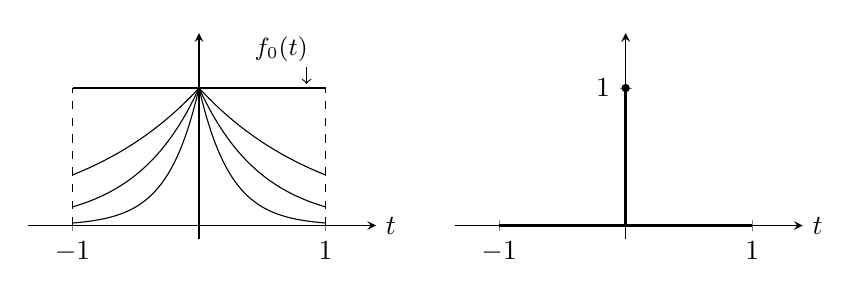
\begin{tikzpicture}
\begin{axis}[name=left,width=6cm,height=4.2cm,axis lines=middle,
  xmin=-1.35,xmax=1.4,ymin=-0.1,ymax=1.4,xtick={-1,1},ytick=\empty,
  xlabel={$t$},clip=false,every axis x label/.style={at={(current axis.right of origin)},anchor=west}]
  \addplot[thick,domain=-1:1] {1};
  \addplot[dashed] coordinates {(-1,0) (-1,1)};
  \addplot[dashed] coordinates {(1,0) (1,1)};
  \foreach \n in {1,2,4} {
    \addplot[domain=-1:1,samples=81] {exp(-\n*abs(x))};
  }
  \node[above,font=\small] at (axis cs:0.65,1.12) {$f_0(t)$};
  \draw[->] (axis cs:0.85,1.15) -- (axis cs:0.85,1.03);
\end{axis}
\begin{axis}[at={(left.east)},anchor=west,xshift=1cm,width=6cm,height=4.2cm,axis lines=middle,
  xmin=-1.35,xmax=1.4,ymin=-0.1,ymax=1.4,xtick={-1,1},ytick={1},
  xlabel={$t$},every axis x label/.style={at={(current axis.right of origin)},anchor=west}]
  \addplot[very thick] coordinates {(-1,0) (1,0)};
  \addplot[very thick] coordinates {(0,0) (0,1)};
  \addplot[only marks,mark=*,mark size=1.3pt] coordinates {(0,1)};
\end{axis}
\end{tikzpicture}
\end{center}
\explain{Left: $f_0, f_1, f_2, f_4$. Right: pointwise limit as $n\to\infty$ ($0$ for $t\neq0$, $1$ at $t=0$) $\notin \V$ (not continuous).}

\begin{center}
\begin{minipage}{0.32\textwidth}
\centering
\begin{tikzpicture}
\begin{axis}[width=4.6cm,height=3.2cm,axis lines=middle,
  xmin=-1.35,xmax=1.4,ymin=-0.3,ymax=1.2,xtick={-1,1},ytick=\empty]
  \addplot[very thick] coordinates {(-1,0) (1,0)};
\end{axis}
\end{tikzpicture}

$0(t)\in\V$
\end{minipage}%
\begin{minipage}{0.64\textwidth}
Candidate limit: the zero function $0(t)$.\\ $v\in\V$ is satisfied \checkmark
\end{minipage}
\end{center}
\begin{align*}
\norm{f_n(t) - 0(t)} &= \norm{f_n(t)} = \int_{-1}^{1}\left|e^{-n|t|}\right|dt\\
&= \int_{-1}^{1} e^{-n|t|}\,dt
&&\text{(exponential is positive)}\\
&= 2\cdot\int_0^1 e^{-nt}\,dt
&&\text{(even function)}\\
&= 2\,\frac{e^{-nt}}{-n}\bigg|_0^1 = -2\left(\frac{e^{-n}}{n} - \frac1n\right)\\
\norm{f_n(t) - 0(t)} &= -\frac{2}{n}\big(\underbrace{e^{-n} - 1}_{\to -1}\big) = \frac{2\,(1-e^{-n})}{n} \le \frac2n\\
\lim_{n\to\infty}\norm{f_n(t) - 0(t)} &= 0 \;\Rightarrow\; \norm{v_n - v}\to 0 \text{ as } n\to\infty \ \checkmark
\end{align*}
$\therefore$ \key{It is convergent to the zero function.}
\end{example}

\needspace{12\baselineskip}
\sep
\key{Convergence depends on the distance definition} (the norm):
\begin{itemize}[nosep]
\item for the $\mathcal{L}_1$ norm $\Rightarrow$ convergent
\item for the $\mathcal{L}_\infty$ (sup) norm $\Rightarrow$ divergent
\end{itemize}
\begin{insight}
With $\norm{f}_\infty = \max_{-1\le t\le 1}|f(t)|$ we get $\norm{f_n - 0}_\infty = \max_t e^{-n|t|} = 1$ (at $t=0$) for every $n$, so $f_n\not\to 0$. No other continuous $g$ works either: $\norm{f_n - g}_\infty\to0$ would force $g(t) = \lim_n f_n(t)$ pointwise, i.e.\ $g(0)=1$ and $g(t)=0$ for $t\neq0$, which is not continuous. The $\mathcal L_1$ norm only ``sees'' area, and the area under the narrowing peak vanishes; the $\mathcal L_\infty$ (sup) norm sees the peak height, which stays $1$.
\end{insight}

\subsection{Cauchy Sequences and Completeness}\label{ss:cauchy}
\begin{definition}
Let $(\V,\F,\norm{\cdot})$ be a normed space. A sequence $\{v_n\}_{n=0}^\infty$ is said to be a \term{Cauchy sequence} iff
\[
\lim_{n,m\to\infty}\norm{v_n - v_m} = 0
\]
\end{definition}
\begin{claim}
\key{Every convergent sequence is a Cauchy sequence.} The reverse statement, in general, is not correct.
\[
\text{Convergent} \;\underset{\not\Leftarrow}{\Rightarrow}\; \text{Cauchy}
\]
\end{claim}
\begin{proof}
Suppose that $\{v_n\}_{n=0}^\infty$ is convergent to $v\in\V$, i.e.\ $\lim_{n\to\infty}\norm{v_n - v} = 0$. Then
\begin{align*}
\lim_{n,m\to\infty}\norm{v_n - v_m} &= \lim_{n,m\to\infty}\norm{v_n - v + v - v_m}\\
&\le \lim_{n,m\to\infty} \big(\norm{v_n - v} + \norm{v - v_m}\big)\\
&= \underbrace{\lim_{n\to\infty}\norm{v_n - v}}_{=0} + \underbrace{\lim_{m\to\infty}\norm{v_m - v}}_{=0} = 0
\end{align*}
\explain{Inequality step: triangle inequality, $\norm{a+b}\le\norm{a}+\norm{b}$ with $a = v_n - v$, $b = v - v_m$.}
\[
0 \le \lim_{n,m\to\infty}\norm{v_n - v_m} \le 0 \;\Rightarrow\; \lim_{n,m\to\infty}\norm{v_n - v_m} = 0 \;\Rightarrow\; \{v_n\} \text{ is Cauchy.}
\qedhere
\]
\end{proof}
% corrected: notes justified the inequality step "by absolute convergence"; it is the triangle inequality (and ||v - v_m|| = ||v_m - v|| by homogeneity with alpha = -1)

% ===== Page 17 =====
\origpage{17}
\begin{example}
$\V = \Q$: set of rational numbers, $\F = \Q$ as well.
\[
\sqrt{2} = 1.41421356237310\ldots \;\Rightarrow\; \text{not a rational number}
\]
\begin{align*}
v_0 &= 1 = \tfrac11\\
v_1 &= 1.4 = \tfrac{14}{10}\\
v_2 &= 1.41 = \tfrac{141}{100}\\
v_3 &= 1.414 = \tfrac{1414}{1000}\\
&\ \,\vdots
\end{align*}
\needspace{7\baselineskip}
We need $v\in\V$ such that $\norm{v_n - v}\to 0$ as $n\to\infty$, where $v_n \in\V\ \forall n$.
But $v$ should be $\sqrt2$ for $\norm{v_n - v}\to 0$ as $n\to\infty$.
\begin{center}
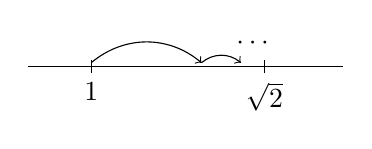
\begin{tikzpicture}
  \draw (0,0) -- (4,0);
  \draw (0.8,0.08) -- (0.8,-0.08) node[below] {$1$};
  \draw (3,0.08) -- (3,-0.08) node[below] {$\sqrt2$};
  \draw[->] (0.8,0.05) to[out=40,in=140] (2.2,0.05);
  \draw[->] (2.2,0.05) to[out=40,in=140] (2.7,0.05);
  \node at (2.85,0.3) {$\cdots$};
\end{tikzpicture}
\end{center}
Since $\sqrt2\notin\V$: $\therefore$ \key{$\{v_n\}$ is not convergent (in $\V$).}

\paragraph{What about Cauchyness?}
\[
\norm{v_n - v_m} \to 0 \text{ as } n,m\to\infty
\]
$v_n$ is actually Cauchy as elements are approaching each other.
\explain{Indeed $v_n$ and $v_m$ agree in the first $\min(n,m)$ decimals, so $|v_n - v_m| < 10^{-\min(n,m)} \to 0$.}
\[
\therefore\ \text{\key{Convergent $\Rightarrow$ Cauchy}} \quad\text{but}\quad \text{Cauchy} \not\Rightarrow \text{Convergent}
\]
\explain{Margin note (Turkish): ``ben bi sequence olsam sana converge ederdim.''}
\end{example}
If a set does not have holes $\Rightarrow$ \key{complete} set.
\begin{insight}
The same sequence viewed in $\V=\R$ converges (to $\sqrt2\in\R$): convergence depends on the space, not only on the terms. $\R$ is complete (it ``fills the holes'' of $\Q$), and so is every finite-dimensional normed space over $\R$ or $\C$, e.g.\ $(\R^n,\norm{\cdot}_p)$. Incompleteness is therefore a phenomenon of infinite-dimensional spaces such as function spaces, as the next example shows.
\end{insight}

\begin{definition}
A normed space is said to be \term{complete} iff \key{every Cauchy sequence is convergent}. A complete normed space is called a \term{Banach space}.
\end{definition}
\begin{example}
A normed space defined as
\[
\V = \left\{ f(\cdot) \;\middle|\; f:[-1,1]\to\R,\ f \text{ is continuous } \& \int_{-1}^{1}|f(t)|\,dt < \infty\right\},
\qquad
\norm{f}_1 = \int_{-1}^{1}|f(t)|\,dt
\]
Consider the sequence $\{f_n\}_{n=1}^\infty$:
\[
f_n(t) = \begin{cases} 1, & -1\le t\le 0\\ 1 - nt, & 0\le t\le \frac1n\\ 0, & \frac1n\le t\le 1\end{cases}
\]
\begin{center}
\pgfplotsset{fnplot/.style={width=4.6cm,height=3.4cm,axis lines=middle,
  xmin=-1.3,xmax=1.35,ymin=-0.15,ymax=1.35,ytick={1},
  yticklabel style={anchor=south west,font=\small},
  every axis y label/.style={at={(current axis.above origin)},anchor=south west}}}
\begin{tikzpicture}
\begin{axis}[fnplot,name=a1,xtick={-1,1},ylabel={$f_1(t)$},xlabel={$t$},
  every axis x label/.style={at={(current axis.right of origin)},anchor=west}]
  \addplot[thick] coordinates {(-1,0) (-1,1) (0,1) (1,0)};
\end{axis}
\begin{axis}[fnplot,name=a2,at={(a1.east)},anchor=west,xshift=0.6cm,
  xtick={-1,0.5,1},xticklabels={$-1$,$\frac12$,$1$},ylabel={$f_2(t)$}]
  \addplot[thick] coordinates {(-1,0) (-1,1) (0,1) (0.5,0) (1,0)};
\end{axis}
\node at ($(a2.east)+(0.35,0)$) {$\cdots$};
\begin{axis}[fnplot,name=a3,at={(a2.east)},anchor=west,xshift=0.7cm,
  xtick={-1,0.25,1},xticklabels={$-1$,$\frac1n$,$1$},ylabel={$f_n(t)$}]
  \addplot[thick] coordinates {(-1,0) (-1,1) (0,1) (0.25,0) (1,0)};
\end{axis}
\end{tikzpicture}
\end{center}
Is the sequence $\{f_n\}$ Cauchy? Convergent?
\[
\norm{f_n(t) - f_m(t)}_1 = \int_{-1}^{1}|f_n(t) - f_m(t)|\,dt
\]
\begin{center}
\begin{minipage}{0.45\textwidth}
\centering
\begin{tikzpicture}
\begin{axis}[width=5.4cm,height=3.8cm,axis lines=middle,
  xmin=-1.3,xmax=1.35,ymin=-0.15,ymax=1.3,ytick={1},yticklabel style={anchor=south west},
  xtick={-1,0.3,0.6,1},xticklabels={$-1$,$\frac1m$,$\frac1n$,$1$},clip=false]
  \addplot[pattern=north east lines,draw=none] coordinates {(0,1) (0.6,0) (0.3,0) (0,1)};
  \addplot[thick] coordinates {(-1,0) (-1,1) (0,1) (0.6,0) (1,0)};
  \addplot[thick] coordinates {(0,1) (0.3,0)};
  \draw (axis cs:0.33,0.45) -- (axis cs:0.75,0.95) node[right,font=\small,align=left] {difference\\integration\\is this area.};
\end{axis}
\end{tikzpicture}
\end{minipage}%
\begin{minipage}{0.5\textwidth}
\[
\text{Area} = \left|\frac1n - \frac1m\right|\cdot\frac12
\]
\explain{Triangle with vertices $(0,1)$, $(\frac1m,0)$, $(\frac1n,0)$: base $|\frac1n-\frac1m|$, height $1$.}
\[
\lim_{n,m\to\infty}\left|\frac1n - \frac1m\right|\cdot\frac12 = 0
\]
\end{minipage}
\end{center}
\begin{center}
\begin{minipage}{0.45\textwidth}
\centering
\begin{tikzpicture}
\begin{axis}[width=5.4cm,height=3.8cm,axis lines=middle,
  xmin=-1.3,xmax=1.35,ymin=-0.15,ymax=1.3,ytick={1},yticklabel style={anchor=south west},
  xtick={-1,0,1},title={$f_n \xrightarrow{\,n\to\infty\,}$},title style={font=\small}]
  \addplot[thick] coordinates {(-1,0) (-1,1) (0,1) (0,0) (1,0)};
\end{axis}
\end{tikzpicture}
\end{minipage}%
\begin{minipage}{0.5\textwidth}
The limit $\notin\V$ (not continuous).

$\Rightarrow \{f_n\}$ is Cauchy but not convergent.

$\therefore$ \key{$(\V,\F,\norm{\cdot}_1)$ is not complete.}
\end{minipage}
\end{center}
\begin{insight}
To be precise, ``not convergent'' means no \emph{continuous} $g$ satisfies $\norm{f_n - g}_1\to 0$. If one did, then on $[-1,0]$ we would need $\int_{-1}^0|1-g|\,dt = 0$, so $g = 1$ there; and on every $[\delta,1]$, $\delta>0$, $f_n = 0$ eventually, so $g = 0$ there. Then $g$ jumps at $t = 0$, contradicting continuity. The ``limit'' is the step function, which lies outside $\V$.
\end{insight}
\end{example}

% ===== Page 18 =====
\origpage{18}
\paragraph{Now with $(\V,\F,\norm{\cdot}_\infty)$.}
\begin{align*}
\norm{f}_\infty &= \max_{-1\le t\le 1}|f(t)|\\
\norm{f_n(t) - f_m(t)}_\infty &= \max_{-1\le t\le 1}|f_n(t) - f_m(t)|
\end{align*}
\begin{center}
\begin{minipage}{0.4\textwidth}
\begin{align*}
f_n(t) &= 1 - nt \quad \big(0\le t\le\tfrac1n\big)\\
f_n\!\left(\tfrac1m\right) &= 1 - \frac nm \quad (m\ge n)
\end{align*}
\end{minipage}%
\begin{minipage}{0.5\textwidth}
\centering
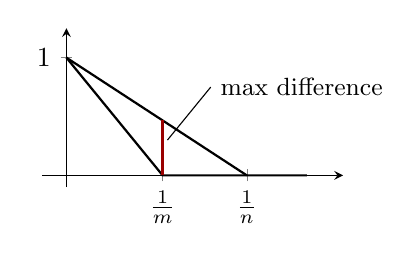
\begin{tikzpicture}
\begin{axis}[width=5.4cm,height=3.6cm,axis lines=middle,
  xmin=-0.1,xmax=1.15,ymin=-0.1,ymax=1.25,ytick={1},
  xtick={0.4,0.75},xticklabels={$\frac1m$,$\frac1n$},clip=false]
  \addplot[thick] coordinates {(0,1) (0.4,0) (1,0)};
  \addplot[thick] coordinates {(0,1) (0.75,0)};
  \addplot[very thick,red!60!black] coordinates {(0.4,0) (0.4,{1-0.4/0.75})};
  \draw (axis cs:0.42,0.3) -- (axis cs:0.6,0.75) node[right,font=\small] {max difference};
\end{axis}
\end{tikzpicture}
\end{minipage}
\end{center}
% corrected: notes wrote lim_{n,m} ||f_n - f_m||_inf = |1 - n/m|; the distance itself equals |1 - n/m| (m >= n), and this does not tend to 0
\begin{align*}
\norm{f_n(t) - f_m(t)}_\infty &= f_n\!\left(\tfrac1m\right) - \underbrace{f_m\!\left(\tfrac1m\right)}_{0} = {\underbrace{\left|1 - \frac nm\right|}_{\neq 0 \text{ unless } n=m}} \qquad (m\ge n)\\
\text{e.g.\ } m = 2n:\quad \norm{f_n - f_{2n}}_\infty &= \tfrac12 \quad \text{for every } n
\end{align*}
\begin{center}
\fbox{\begin{minipage}{0.75\textwidth}\small\itshape
$n$ ve $m$'in nasıl $\infty$'a gittiği fark etmez, her zaman limit sonucu sıfır olmalı. Bu senaryoda if $n=m$ o zaman limit sıfır, onun dışında değil.
\end{minipage}}
\end{center}
% translation: it does not matter how n and m go to infinity, the limit must always be zero.
% In this scenario the limit is zero only if n = m, not otherwise.
\explain{It does not matter how $n$ and $m$ go to $\infty$; the limit must always be zero. Here it is zero only if $n=m$.}
\explain{The maximum is at $t=\frac1m$: on $[0,\frac1m]$ the difference $(m-n)t$ increases, and on $[\frac1m,\frac1n]$ it equals $1-nt$, which decreases.}
$\therefore$ \key{$\{f_n\}$ is not Cauchy} in the sup norm.
